\documentclass[12pt]{book}
\usepackage[utf8]{inputenc}
\usepackage[T1]{fontenc}
\usepackage{mathptmx}
\usepackage{geometry}
\usepackage{mathtools}
\usepackage[english]{babel}
\usepackage{graphicx}
\usepackage{subcaption}
\usepackage{stackengine}
\usepackage[os=win]{menukeys}
\usepackage{hyperref}
\usepackage{xcolor}
\usepackage{tikz}
\usepackage[yyyymmdd,hhmmss]{datetime}
\usepackage{etoolbox}
\usepackage[inline]{enumitem}
\usepackage{pdfpages}

\newcommand{\WindowsLogo}{\raisebox{-0.1em}{
\includegraphics[height=0.8em]{images/logo/Windows_3_logo_simplified}}}
%\newcommand{\PowerLogo}{\raisebox{-0.1em}{
\includegraphics[height=0.8em]{images/logo/power}}}
\newcommand{\WinKey}{\keys{\WindowsLogo}}
\newcommand{\PowerKey}{\keys{\PowerLogo}}

\patchcmd{\thebibliography}{\section*{\refname}}{}{}{}

\addto\captionsenglish{\renewcommand{\contentsname}{Daftar Isi}}
\addto\captionsenglish{\renewcommand{\figurename}{Gambar}}

\hypersetup{
	colorlinks=true, %set true if you want colored links
	linktoc=all,     %set to all if you want both sections and subsections linked
	linkcolor=blue,  %choose some color if you want links to stand out
	urlcolor=blue,   %url color
}

\geometry{
	a4paper,
	left=10mm,
	right=10mm,
	top=15mm,
	bottom=15mm,
}

\date{}

\hypersetup{citecolor=black}

\definecolor{LightGray}{gray}{0.95}

%\pagecolor[rgb]{0.1,0.1,0.1}
%\color[rgb]{1,1,1}

\begin{document}

	\frontmatter
	\begin{titlepage}
		\centering
		{\LARGE \bf Panduan Dasar Draft PCB Menggunakan KiCAD}
		\vfill
		{\Large Achmadi ST MT}
		\vfill
		
\includegraphics[width=250pt]{images/logo/logoviblab}
		\vfill
		\vfill
	\end{titlepage}

	%%%%%%%%%%%%%%%%%%%%%%%%%%%%%%%%%%%%%%%%%%%%%%%%%%%%%%%%%%%%%%%%%

	\newpage
	\tableofcontents

	%%%%%%%%%%%%%%%%%%%%%%%%%%%%%%%%%%%%%%%%%%%%%%%%%%%%%%%%%%%%%%%%%

	%%%%%%%%%%%%%%%%%%%%%%%%%%%%%%%%%%%%%%%%%%%%%%%%%%%%%%%%%%%%%%%%%

	\newpage
	\chapter{Penggunaan Buku}

	\section{Umum}
	Buku ini dibuat dengan tujuan penggunaan utama sebagai panduan digital untuk mempermudah search dan copy-paste.
	Anda tidak perlu mencetak buku ini ke bentuk kertas.
	Seluruh navigasi buku ini diharapkan menggunakan klik ke hyperlink di Daftar Isi,
	atau menggunakan tampilan \textbf{Index} yang tersedia di \textbf{SideBar} program pembaca PDF yang anda gunakan.

	\section{Petunjuk}
	Beberapa petunjuk yang digunakan di buku ini:
	\begin{itemize}
		\item \textbf{Cetak Tebal}: Menginformasikan identifier (keyword, variabel, fungsi, alamat, nama file, dst) yang berada di suatu paragraf
		\item \textit{Cetak Miring}: Bersama simbol panah (->) dan simbol lain, menginformasikan langkah-langkah klik menu/tombol.
		\item \textbf{TIPS:} Menginformasikan hal-hal yang dapat membantu atau pengetahuan tambahan.
		\item \textbf{PERINGATAN:} Menginformasikan hal-hal yang bener-benar harus diperhatikan.
	\end{itemize}

	%%%%%%%%%%%%%%%%%%%%%%%%%%%%%%%%%%%%%%%%%%%%%%%%%%%%%%%%%%%%%%%%%

	\newpage
	\mainmatter
	\chapter{Program KiCAD}

	\section{Pengenalan}

	KiCAD adalah paket software EDA (Electronic Design Automation) yang dikembangkan untuk perancangan papan sirkuit elektronik tercetak (Printed Circuit Board atau PCB)
	secara professional yang bersifat gratis dan terbuka.

	KiCAD dapat disandingkan dengan perangkat perancangan PCB professional lain seperti Altium, Diptrace, EasyEDA, dan lainnya.
	KiCAD tersedia untuk sistem operasi Windows, GNU/Linux, dan MacOS.\\

	Berikut adalah tampilan 4 software utama dalam paket software KiCAD:
	\begin{figure}[!ht]
		\centering
		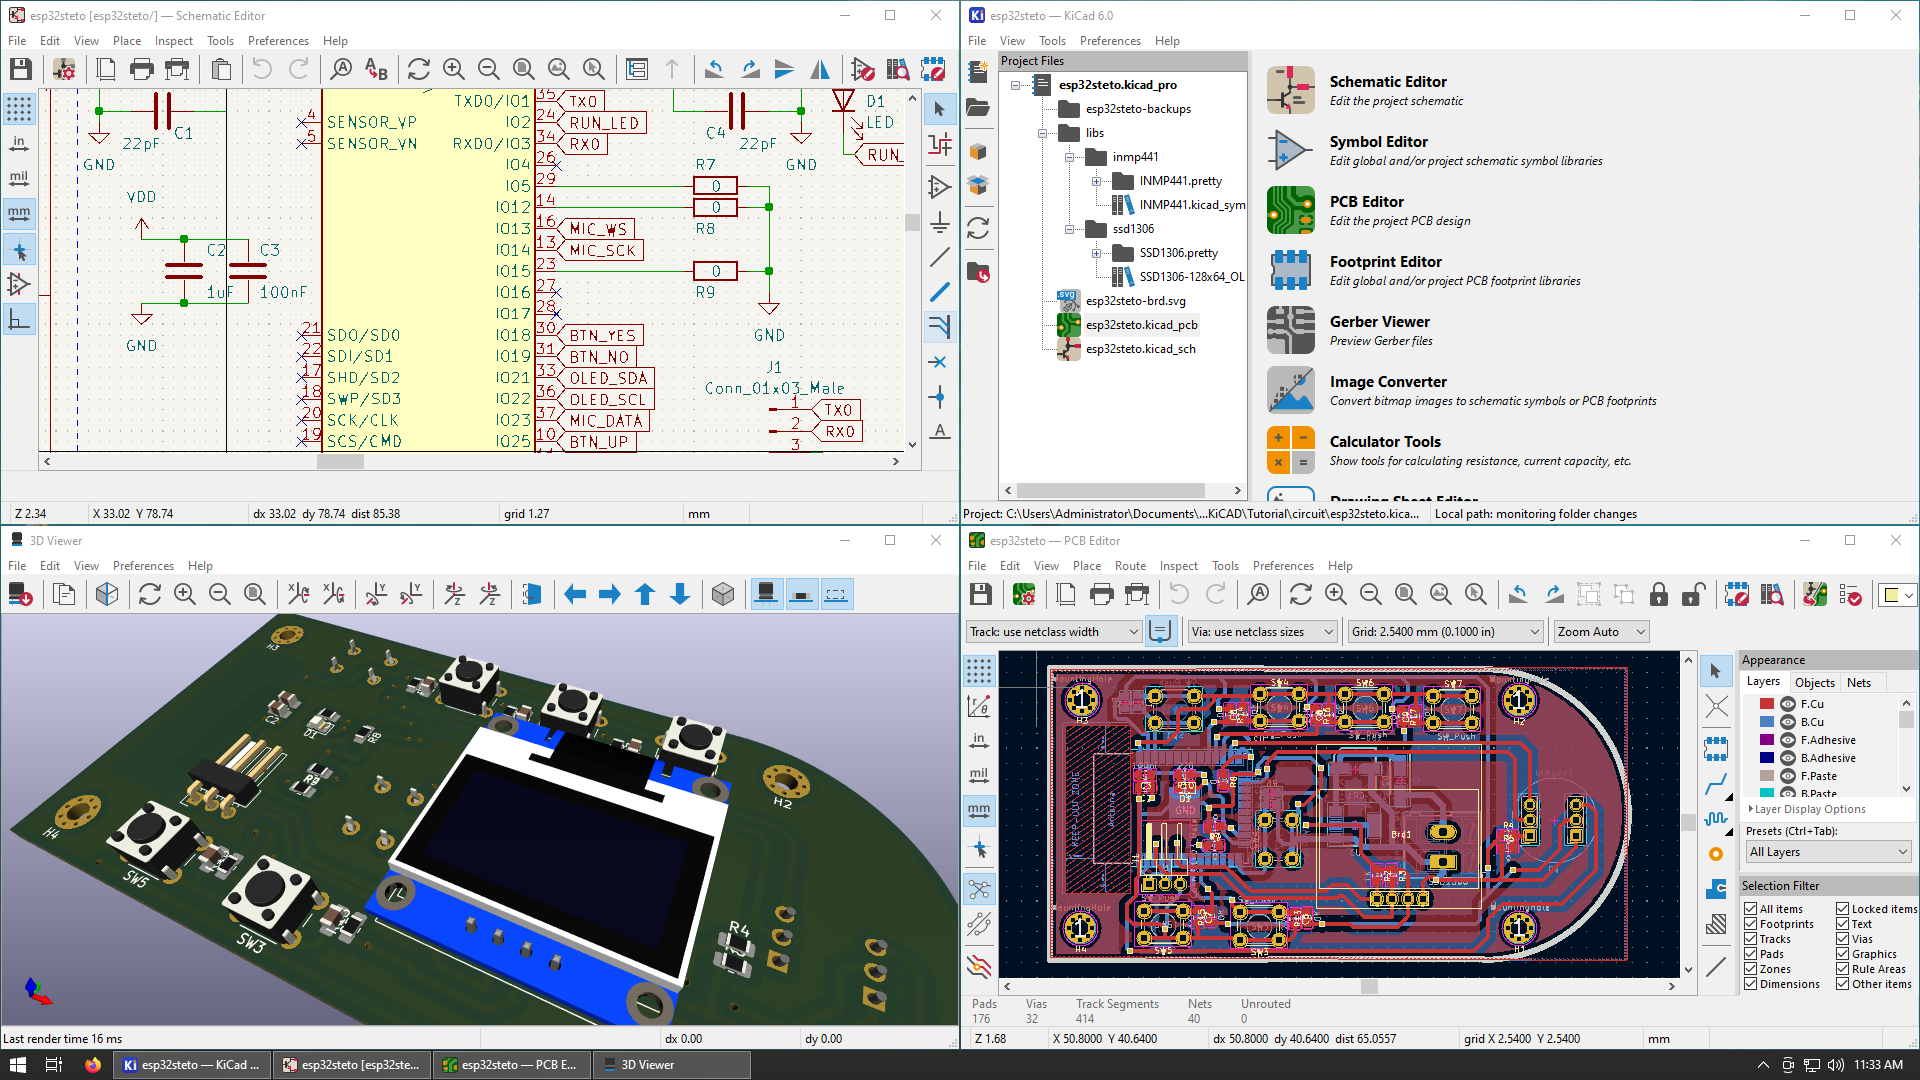
\includegraphics[width=\textwidth]{images/kicad_windows10}
		\caption{Tampilan KiCAD Windows 10}
	\end{figure}

	\textbf{TIPS:} Sepanjang tutorial, akan digunakan tampilan Windows 10 atau GNU/Linux sebagai acuan.
	Namun tutorial yang sama akan dapat pula digunakan di sistem operasi lain seperti Windows 8 dan Windows 11.\\

	\textbf{PERINGATAN:} Versi KiCAD yang akan digunakan adalah versi 6, dimana untuk sistem operasi Windows
	hanya bisa diinstal di Windows 8 dan selanjutnya.
	Untuk pengguna Windows 7 dan sebelumnya, disarankan menggunakan KiCAD versi 5.

	\newpage
	\section{Instalasi}

	\subsection{GNU/Linux}

	\subsection{Windows}

	\subsection{MacOS}

	Nanti akan dilengkapi saat penulis cukup berduit untuk memiliki laptop Apple dan MacOS



\end{document}